\chapter{Results and Discussion}
% ADVISER COMMENT (DON'T DELETE,2025-05-30): need to have 2-3 sentences as an intro
% ADVISER COMMENT (DON'T DELETE,2025-05-30): general comment: cite only the first mention of Mr. Basanes in the chapter, no need to keep citing him in the rest of the chapter.
% ADVISER COMMENT (DON'T DELETE,2025-05-30): general comment: need to rewrite appendix references that are in parenthesis. EX: The model did lose the third game within just 32 moves (see Appendix B.2) -> can be rewritten as "The model did lose the third game within just 32 moves. The full moves of the game can be seen in Appendix B.2."

This chapter presents the results found after model generation and evaluation and discusses the findings synthesized from it. This chapter presents the training results of the model generation and discusses the average loss of the generated models. This chapter also analyzes the evaluation of the final best model against previous best models and the analysis of Mr. Basanes (\textit{personal communications}, May 13-23, 2025) of the best model by playing ten rounds against it.

\section{Training Results}

A total of 100,000 games were played over 20 iterations during model generation. The average training loss for each iteration and the wins, draws, and losses against the previous best model for 100 games are shown in Figure \ref{fig:training-results}. The curve shown in Figure \ref{fig:train-loss-per-iteration} has the average training loss as the vertical axis and the number of iterations as the horizontal axis. The bar graph shown in Figure \ref{fig:train-wdl-per-iteration} has the ratio of wins, draws and losses against the previous model for 100 games as the vertical axis and the number of iterations as the horizontal axis.

\pgfplotstableread{
I  W  D L
1  66 0 34
2  53 0 47
3  54 0 46
4  60 0 40
5  59 0 41
6  59 0 41
7  60 0 40
8  48 0 52
9  48 0 52
10 46 0 54
11 56 0 44
12 61 0 39
13 53 0 47
14 49 0 51
15 51 0 49
16 50 0 50
17 51 0 49
18 51 0 49
19 68 0 32
20 49 0 51
}\wdltraindata

\begin{figure}[H]
    \centering
    \begin{subfigure}{0.4\textwidth}
        \centering
        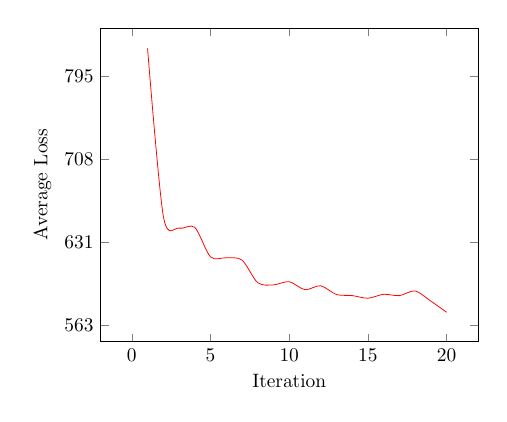
\begin{tikzpicture}[scale=0.7]
          \begin{axis}[
            xmin = -2, xmax = 22,
            ymin = 550, ymax = 850,
            ymode = log, log ticks with fixed point,
            xlabel = Iteration,
            ylabel = Average Loss]
            \addplot[smooth, red] plot coordinates {
                (1 , 826.237610)
                (2 , 654.909119)
                (3 , 644.004456)
                (4 , 644.672119)
                (5 , 618.844055)
                (6 , 618.023010)
                (7 , 616.063965)
                (8 , 597.026978)
                (9 , 595.188477)
                (10, 597.854187)
                (11, 591.271484)
                (12, 594.479980)
                (13, 587.326843)
                (14, 586.461426)
                (15, 584.299072)
                (16, 587.507446)
                (17, 586.405396)
                (18, 590.255615)
                (19, 581.949158)
                (20, 573.042419)
            };
          \end{axis}
        \end{tikzpicture}
        \caption{Average Loss Over Iteration}
        \label{fig:train-loss-per-iteration}
    \end{subfigure}
    \begin{subfigure}{0.4\textwidth}
        \centering
        \begin{tikzpicture}[scale=0.7]
          \begin{axis}[
            ybar stacked,
            bar width=7pt,
            xmin = -2, xmax = 22,
            ymin = 0, ymax = 100,
            xlabel = Iteration]
            \draw (0,60) -- (300,60);
            \addplot[fill=green!50] table [y = W, meta = I] {\wdltraindata};
            \addlegendentry{Win}
            \addplot[fill=blue!50] table [y = D, meta = I] {\wdltraindata};
            \addlegendentry{Draw}
            \addplot[fill=red!50] table [y = L, meta = I] {\wdltraindata};
            \addlegendentry{Loss}
          \end{axis}
        \end{tikzpicture}
        \caption{Win-Draw-Loss Over Iteration}
        \label{fig:train-wdl-per-iteration}
    \end{subfigure}
    \caption{Training Results of the Model Generation}
    \label{fig:training-results}
\end{figure}

As shown in Figure \ref{fig:train-loss-per-iteration}, the average loss of the model continuously decreased as the number of iterations increased. This shows that the model is learning to accurately predict the WDL probability and the policy vector according to the MCTS algorithm of a given state. Only five models became the best model during the 20 iterations of model generation, as shown in Figure \ref{fig:train-wdl-per-iteration} where only five iterations have reached the 60 number of wins line. This shows that a new best model is not generated every iteration.

% The models that surpassed 60 combined wins and draws per iteration becomes the next best model, as shown in Table \ref{tab:train-best-models-version-per-iteration}.

% \begin{table}[H]
%     \centering
%     \begin{tabular}{ccc}
%         \hline
%         Version & Iteration & Wins Against the Previous Version \\ \hline
%         v1      & 1         & 66                                \\
%         v2      & 4         & 60                                \\
%         v3      & 7         & 60                                \\
%         v4      & 12        & 61                                \\
%         v5      & 19        & 68                                \\ \hline
%     \end{tabular}
%     \caption{Versions of Trained Best Models and their Iterations}
%     \label{tab:train-best-models-version-per-iteration}
% \end{table}

% The new versions of the best model are better against the previous versions of the best model, as shown by the number of wins they got against the previous versions of the best model, as shown in Table \ref{tab:train-best-models-version-per-iteration}.

\section{Final Best Model Against Previous Best Models}

The previous versions of the best model were pitted against the final version of the best model for 100 games each with 100 MCTS simulations for each move to assess the competence of the final version of the best model. The wins, draws and losses of the previous best models against the final version of the best model are recorded as shown in Figure \ref{fig:wdl-eval}.

\pgfplotstableread{
V  W  D L
v1 27 0 73
v2 33 0 67
v3 43 0 57
v4 49 0 51
v5 54 0 46
}\wdlevaldata
    
\begin{figure}[H]
    \centering
    \begin{tikzpicture}
      \begin{axis}[
        ybar stacked,
        xtick = data,
        ymin = 0, ymax = 100,
        xtick = data,
        xticklabels from table={\wdlevaldata}{V},
        xlabel = Version]
        \addplot[fill=green!50] table [y = W, meta = V, x expr=\coordindex] {\wdlevaldata};
        \addlegendentry{Win}
        \addplot[fill=blue!50] table [y = D, meta = V, x expr=\coordindex] {\wdlevaldata};
        \addlegendentry{Draw}
        \addplot[fill=red!50] table [y = L, meta = V, x expr=\coordindex] {\wdlevaldata};
        \addlegendentry{Loss}
      \end{axis}
    \end{tikzpicture}
    \caption{Win-Draw-Loss of the Previous Best Models Against the Best Model}
    \label{fig:wdl-eval}
\end{figure}

An increasing trend is seen in the number of wins that the previous best models make against the final best model. This trend shows the improvement in model competence after the training phase of each iteration. The final best model won 54 of 100 games competing against itself. According to Mr. Basanes, the first player in the game of Damath has an advantage over the second player, since the second player has to catch up with the moves of the first player. The final version of the model wins more than half of the games, since a Damath player competing against a player of similar skills and experience may win more if they were the first player, and the model evaluation picks a random initial player for the hundred of games played against each evaluation.

\section{Best Model Against an Expert Damath Player}

To further analyze the competence of the final version of the best model, we let it play against Mr. Basanes for ten games. Mr. Basanes won seven out of ten games against this model. Mr. Basanes plays as the red player, while this model plays as the black player. In this section, the researchers discuss the moves chosen by this model that showed strategies worth analyzing according to Mr. Basanes.

% \subsection{First Game Against an Expert Damath Player}

For the first game, the model plays first with 500 MCTS simulations. The full moves of this game can be seen on Appendix \ref{tab:first-game}. The model sets up an elaborate trap by letting Mr. Basanes capture pieces that temporarily gave him an advantage during the first nine moves of the game, as shown in Figure \ref{fig:4-9-game1}. The model forced Mr. Basanes to capture the $0$ piece, setting up a trap that puts the model in a more advantageous position.

\begin{figure}[H]
    \centering
    \begin{subfigure}{0.3\textwidth}
        \centering
        \includegraphics[width=\textwidth]{images/games/game1/move_5.png}
        \caption*{Move 4: A = 0 \textbar\ H = $-15$}
    \end{subfigure}
    \quad
    \begin{subfigure}{0.3\textwidth}
        \centering
        \includegraphics[width=\textwidth]{images/games/game1/move_6.png}
        \caption*{Move 5: A = 0 \textbar\ H = $-15$}
    \end{subfigure}
    \quad
    \begin{subfigure}{0.3\textwidth}
        \centering
        \includegraphics[width=\textwidth]{images/games/game1/move_7.png}
        \caption*{Move 6: A = 0 \textbar\ H = $-27$}
    \end{subfigure} \\
    \begin{subfigure}{0.3\textwidth}
        \centering
        \includegraphics[width=\textwidth]{images/games/game1/move_8.png}
        \caption*{Move 7: A = 0 \textbar\ H = 54}
    \end{subfigure}
    \quad
    \begin{subfigure}{0.3\textwidth}
        \centering
        \includegraphics[width=\textwidth]{images/games/game1/move_9.png}
        \caption*{Move 8: A = 0 \textbar\ H = 54}
    \end{subfigure}
    \quad
    \begin{subfigure}{0.3\textwidth}
        \centering
        \includegraphics[width=\textwidth]{images/games/game1/move_10.png}
        \caption*{Move 9: A = 0 \textbar\ H = 45}
    \end{subfigure}
    \caption{Fourth to Ninth Moves of the First Game Against an Expert Damath Player} % ADVISER COMMENT (DON'T DELETE): need to specify which "game" this 9 moves are from
    \label{fig:4-9-game1}
\end{figure}

This made the model play the tenth move as shown in Figure \ref{fig:10-game1}. The model was able to make Mr. Basanes have his $-9$ piece captured by the $-9$ piece of the model on a multiply operator on the tenth move. This gave the model a higher score compared to Mr. Basanes. This puts the model at an advantage higher than that of Mr. Basanes and makes the model more likely to win the game.

\begin{figure}[H]
    \centering
    \begin{subfigure}{0.3\textwidth}
        \centering
        \includegraphics[width=\textwidth]{images/games/game1/move_11.png}
        \caption*{Move 10: A = 99 \textbar\ H = 45}
    \end{subfigure}
    \caption{Tenth Move of the First Game Against an Expert Damath Player}
    \label{fig:10-game1}
\end{figure}

According to Mr. Basanes, the model uses the same sequence of opening moves that he discovered to trap players for the early game. The opening sequence of moves that the model played was a solid start to the game of Damath and can lead to eventually winning the game according to Mr. Basanes.

However, Mr. Basanes found a way to gain advantage against the model in the 44th move of the game, as shown in Figure \ref{fig:44-46-game1}. Mr. Basanes made the model capture his 10 dama piece using the model's $-7$ piece on a multiply operator, giving the model an added score of $-140$. Mr. Basanes was able to reverse the situation and eventually win against the model for the first game. 

\begin{figure}[H]
    \centering
    \begin{subfigure}{0.3\textwidth}
        \centering
        \includegraphics[width=\textwidth]{images/games/game1/move_45.png}
        \caption*{Move 44:  A = 83.75 \textbar\ H = 77.5}
    \end{subfigure}
    \quad
    \begin{subfigure}{0.3\textwidth}
        \centering
        \includegraphics[width=\textwidth]{images/games/game1/move_46.png}
        \caption*{Move 45: A = 83.75 \textbar\ H = 77.5}
    \end{subfigure}
    \quad
    \begin{subfigure}{0.3\textwidth}
        \centering
        \includegraphics[width=\textwidth]{images/games/game1/move_47.png}
        \caption*{Move 46: A = $-56.25$ \textbar\ H = 77.5}
    \end{subfigure}
    \caption{44th to 46th Moves of the First Game Against an Expert Damath Player}
    \label{fig:44-46-game1}
\end{figure}

According to Mr. Basanes, the model is a competent player overall but fails to think more ahead of the game on the mid-to-late game. He said that the model sees the traps he sets up in the early game but fails to do so for the remainder of the game. This shows that the model exhibits strong early game strategies, but fails to maintain its position during the mid-to-late game of Damath. 

% This game highlights that model is weak on the end game but strong on the early game as noted by Mr. Basanes . This may be due to the lack of MCTS simulations during the self-play data generation in Algorithm \ref{alg:data-generation}. Which inhibits the model from being able to simulate the outcome of each of its possible moves. The relative strength in the early game may be due 

% \subsection{Second Game Against an Expert Damath Player}

For the second game, Mr. Basanes plays first with the model playing with 500 MCTS simulations. The model was forced to make his $0$ piece a dama piece, as shown in Figure \ref{fig:9-14-game2}. Mr. Basanes took advantage of having to capture first, forcing the model to continuously make capture moves with the 0 dama piece. The full moves of this game can be seen in Appendix \ref{tab:second-game}.

\begin{figure}[H]
\centering
    \begin{subfigure}{0.3\textwidth}
        \centering
        \includegraphics[width=\textwidth]{images/games/game2/move_10.png}
        \caption*{Move 9: H = $0.\overline1$ \textbar\ A = $-4$ \\ W: 0.02 D: 0.00 L: 0.98}
    \end{subfigure}
    \quad
    \begin{subfigure}{0.3\textwidth}
        \centering
        \includegraphics[width=\textwidth]{images/games/game2/move_11.png}
        \caption*{Move 10: H = $0.\overline1$ \textbar\ A = $-4$ \\ W: 0.31 D: 0.00 L: 0.69}
    \end{subfigure}
    \quad
    \begin{subfigure}{0.3\textwidth}
        \centering
        \includegraphics[width=\textwidth]{images/games/game2/move_12.png}
        \caption*{Move 11: H = $0.\overline1$ \textbar\ A = $-4$ \\ W: 0.00 D: 0.00 L: 1.00}
    \end{subfigure} \\
    \begin{subfigure}{0.3\textwidth}
        \centering
        \includegraphics[width=\textwidth]{images/games/game2/move_13.png}
        \caption*{Move 12: H = $0.\overline1$ \textbar\ A = $-4$ \\ W: 0.75 D: 0.00 L: 0.25}
    \end{subfigure}
    \quad
    \begin{subfigure}{0.3\textwidth}
        \centering
        \includegraphics[width=\textwidth]{images/games/game2/move_14.png}
        \caption*{Move 13: H = $0.\overline1$ \textbar\ A = $-4$ \\ W: 0.27 D: 0.00 L: 0.73}
    \end{subfigure}
    \quad
    \begin{subfigure}{0.3\textwidth}
        \centering
        \includegraphics[width=\textwidth]{images/games/game2/move_15.png}
        \caption*{Move 14: H = $0.\overline1$ \textbar\ A = $-4$ \\ W: 0.98 D: 0.00 L: 0.02}
    \end{subfigure} \\
    \caption{Ninth to Fourteenth Moves of the Second Game Against an Expert Damath Player}
    \label{fig:9-14-game2}
\end{figure}

According to Mr. Basanes having a 0 dama piece in this position is disadvantageous and may lead to losing the game if not removed immediately because it is trapped. The model accurately predicted that having the 0 dama piece made it likely to lose the third game according to the WDL predictions in Figure \ref{fig:9-14-game2}. The prediction made by the model and Mr. Basanes turns out to be correct. The model lost the third game within just 32 moves, the full moves of this game can be seen in Appendix \ref{tab:second-game}.

% We suspect that during the generation of self-play data, as shown in Algorithm \ref{alg:data-generation}, the model was unable to explore this line of game moves due to the low number of MCTS simulations being 100, which ultimately led to its loss.

% \subsection{Third Game Against an Expert Damath Player}

In the third game, the model plays first with 1000 MCTS simulations (see Appendix \ref{tab:third-game}). Mr. Basanes and the model played the same initial moves as in the first game up to the first 13 moves. The model made different moves afterwards due to the increase in the number of MCTS simulations. This made the model consider more steps ahead before making a move.

After the 36th move of the third game, the model appears to be winning as it has a higher score of 107 compared to the score of Mr. Basanes of 68.5, as shown in Figure \ref{fig:36-38-game3}. However, the WDL predictions of the model indicate that Mr. Basanes is more likely to win based on the current state of the game instead. However, the 37th move of Mr. Basanes caused the WDL predictions of the model to suddenly reverse.  

\begin{figure}[H]
    \centering
    \begin{subfigure}{0.3\textwidth}
        \centering
        \includegraphics[width=\textwidth]{images/games/game3/move_37.png}
        \caption*{Move 36: H = 68.5 \textbar\ A = 107 \\ W: 0.86 D: 0.00 L: 0.14}
    \end{subfigure}
    \quad
    \begin{subfigure}{0.3\textwidth}
        \centering
        \includegraphics[width=\textwidth]{images/games/game3/move_38.png}
        \caption*{Move 37:  H = 68.5 \textbar\ A = 107\\ W: 0.26 D: 0.00 L: 0.74}
    \end{subfigure}
    \quad
    \begin{subfigure}{0.3\textwidth}
        \centering
        \includegraphics[width=\textwidth]{images/games/game3/move_39.png}
        \caption*{Move 38:  H = 68.5 \textbar\ A = 116 \\ W: 0.08 D: 0.00 L: 0.92}
    \end{subfigure}
    \caption{36th to 38th Moves of the Third Game Against an Expert Damath Player}
    \label{fig:36-38-game3}
\end{figure}

This indicates that Mr. Basanes has chosen a wrong 37th move according to the model. The model accurately predicted that the move was indeed a bad move, as Mr. Basanes eventually lost the third game. After the third game, we asked Mr. Basanes to review the moves he made and to figure out why he lost the game. We informed Mr. Basanes of the model's prediction for his 37th move and made him re-analyze his moves. 

To analyze whether the WDL prediction of the model works correctly, we let Mr. Basanes play the same initial moves of the third game and let him play a different 37th move that might have led to him winning the game. Mr. Basanes pointed out a better move as shown in Figure \ref{fig:36-38-game3b}. The WDL predictions of the model agree with this move. We let Mr. Basanes continue this alternate third game and it actually led to Mr. Basanes winning the game. The full moves of the alternate third game can be seen in Appendix \ref{tab:alt-third-game}.

% ADVISER COMMENT (DON'T DELETE): remove this result as it is already skewed since Mr. Basanes already lost and this is like giving a "rewind" ability

% RESEARCHERS' REPLY: we would like to continue adding the results of the alternative moves for the third game to show that WDL predictions of the model is accurate in predicting the outcome of the game

% ADVISER COMMENT (DON'T DELETE,2025-05-30): need to clearly state your intent for the "rewind" ability in the content to make it clear to the reader why this was allowed

% RESERCHERS' REPLY: we added the intent of better analyzing whether the WDL prediction of the model works correctly to the first sentence of the paragraph to show intent. also, we paraphrased the paragraph a bit as we would like to show that this is not a rewind ability per se, but an alternative third game where we let mr. basanes play the same initial moves of the third and let him play diffenently for the 37th move going forward to show whether the WDL predictions of the model would be correct.

\begin{figure}[H]
    \centering
    \begin{subfigure}{0.3\textwidth}
        \centering
        \includegraphics[width=\textwidth]{images/games/game3b/move_37.png}
        \caption*{Move 36: H = 68.5 \textbar\ A = 107 \\ W: 0.86 D: 0.00 L: 0.14}
    \end{subfigure}
    \quad
    \begin{subfigure}{0.3\textwidth}
        \centering
        \includegraphics[width=\textwidth]{images/games/game3b/move_38.png}
        \caption*{Move 37: H = 68.5 \textbar\ A = 107 \\ W: 0.26 D: 0.00 L: 0.74}
    \end{subfigure}
    \quad
    \begin{subfigure}{0.3\textwidth}
        \centering
        \includegraphics[width=\textwidth]{images/games/game3b/move_39.png}
        \caption*{Move 38: H = 68.5 \textbar\ A = 105.75 \\ W: 0.82 D: 0.00 L: 0.18}
    \end{subfigure}
    \caption{36th to 38th Moves of the Third Game Against an Expert Damath Player}
    \label{fig:36-38-game3b}
\end{figure}

This shows that the model is capable of predicting the outcome of a game based on the current state of the game. This includes the positions of the pieces on the board and the current scores of the players, and whether making a bad move leads to a losing game. According to Mr. Basanes (\textit{personal connections}, May 13, 2025), he lost the third game because he failed to notice other advantageous pieces to move during the 37th move. He said he was focusing more on the top right corner of the board, which he deemed the most active part of the board.

% An accurate prediction of whether a given state after an arbitrary move would win or not is essential for the truncated rollout of the MCTS algorithm.

In the fourth game, the model plays first with $1000$ MCTS simulations (see Appendix \ref{tab:fourth-game}). According to Mr. Basanes, he made a bad move in the eighth move, as shown in Figure \ref{fig:7-9-game4}. Mr. Basanes allowed his 6 piece to be captured by the model's $-3$ piece thinking that it was just a single capture move. However, he said that he did not notice that it was a double capture move. This put Mr. Basanes in a disadvantageous position compared to the model.

\begin{figure}[H]
\centering
    \begin{subfigure}{0.3\textwidth}
        \centering
        \includegraphics[width=\textwidth]{images/games/game4/move_7.png}
        \caption*{Move 7: A = 6 \textbar\ H = $-54$}
    \end{subfigure}
    \quad
    \begin{subfigure}{0.3\textwidth}
        \centering
        \includegraphics[width=\textwidth]{images/games/game4/move_8.png}
        \caption*{Move 8: A = 6 \textbar\ H = $-54$}
    \end{subfigure}
    \quad
    \begin{subfigure}{0.3\textwidth}
        \centering
        \includegraphics[width=\textwidth]{images/games/game4/move_9.png}
        \caption*{Move 9: A = 9 \textbar\ H = $-54$}
    \end{subfigure} 
    \caption{7th to 9th Moves of the Fourth Game Against an Expert Damath Player}
    \label{fig:7-9-game4}
\end{figure}

This allowed the model to set up a trap that resulted in a score of 77 on the sixteenth move, as shown in Figure \ref{fig:14-17-game4}. The WDL predictions of the model for Mr. Basanes reverse because of this. The model considers Mr. Basanes to be winning during the 14th move. However, after the capture made by the model, the model predicted that Mr. Basanes would lose the game based on the current state of the game.

\begin{figure}[H]
\centering
    \begin{subfigure}{0.3\textwidth}
        \centering
        \includegraphics[width=\textwidth]{images/games/game4/move_14.png}
        \caption*{Move 14: A = 12 \textbar\ H = $-54$ \\ W: 0.01 D: 0.00 L: 0.99}
    \end{subfigure}
    \quad
    \begin{subfigure}{0.3\textwidth}
        \centering
        \includegraphics[width=\textwidth]{images/games/game4/move_16.png}
        \caption*{Move 16: A = 12 \textbar\ A = $-49$ \\ W: 0.99 D: 0.00 L: 0.01}
    \end{subfigure}
    \quad
    \begin{subfigure}{0.3\textwidth}
        \centering
        \includegraphics[width=\textwidth]{images/games/game4/move_17.png}
        \caption*{Move 17: A = 89 \textbar\ A = $-49$ \\ W: 0.77 D: 0.00 L: 0.23}
    \end{subfigure}
    \caption{14th to 17th Moves of the Fourth Game Against an Expert Damath Player}
    \label{fig:14-17-game4}
\end{figure}

This shows that the model is capable of taking advantage of an opponent's bad move. Both Mr. Basanes and the model were able to recognize that the eighth move is a bad move, as highlighted by the WDL predictions of the model for the 14th to 17th moves. This puts the model in an advantageous position, allows it to set up a trap, and gets a higher score compared to Mr. Basanes. According to him, this kind of play was indeed akin to that of a competent human player.

However, the model made an erroneous move during the 36th move according to Mr. Basanes, as shown in \ref{fig:35-37-game4} of the game. The model let Mr. Basanes force it to capture the 0 dama piece of Mr. Basanes with it's $-7$ piece on a minus operator. This force the model to make the bad capture and lose $-14$ points. For the rest of the game, the model allowed Mr. Basanes to force it to make similar bad capture moves.

\begin{figure}[H]
\centering
    \begin{subfigure}{0.3\textwidth}
        \centering
        \includegraphics[width=\textwidth]{images/games/game4/move_35.png}
        \caption*{Move 35: A = 89 \textbar\ H = -19}
    \end{subfigure}
    \quad
    \begin{subfigure}{0.3\textwidth}
        \centering
        \includegraphics[width=\textwidth]{images/games/game4/move_36.png}
        \caption*{Move 36: A = 89 \textbar\ H = -19}
    \end{subfigure}
    \quad
    \begin{subfigure}{0.3\textwidth}
        \centering
        \includegraphics[width=\textwidth]{images/games/game4/move_37.png}
        \caption*{Move 37: A = 75 \textbar\ A = -19}
    \end{subfigure}
    \caption{35th to 37th Moves of the Fourth Game Against an Expert Damath Player}
    \label{fig:35-37-game4}
\end{figure}

According to Mr. Basanes, the model shows a behavior similar to the initial games. The model showed strong strategies during the early game. The model was able to set up a trap that put it in an advantageous position compared to Mr. Basanes for the fourth game. However, the model is still weak during the mid-to-late game. It allowed Mr. Basanes to force it to make bad capture moves for the mid-to-late game of the fourth game and made it eventually lose the game even though it started from an advantageous position.

In the fifth game, the model plays first with 1000 MCTS simulations for each move. Throughout the game up to the last few moves, the model has a higher score compared to Mr. Basanes. The full moves of this game can be seen on Appendix \ref{tab:fifth-game}. The model was stuck at its last move and has no legal actions left except for a move that allows Mr. Basanes to capture its 10 piece with his 8 piece on a multiplier operator, as shown in Figure \ref{fig:40-42-game5}.

\begin{figure}[H]
    \centering
    \begin{subfigure}{0.3\textwidth}
        \centering
        \includegraphics[width=\textwidth]{images/games/game5/move_40.png}
        \caption*{Move 40: A = 90.9 \textbar\ H = 73.79}
    \end{subfigure}
    \quad
    \begin{subfigure}{0.3\textwidth}
        \centering
        \includegraphics[width=\textwidth]{images/games/game5/move_41.png}
        \caption*{Move 41: A = 90.9 \textbar\ H = 73.79}
    \end{subfigure}
    \quad
    \begin{subfigure}{0.3\textwidth}
        \centering
        \includegraphics[width=\textwidth]{images/games/game5/move_42.png}
        \caption*{Move 42: A = 79.9 \textbar\ H = 149.79}
    \end{subfigure}
    \caption{40th to 42th Moves of the Fifth Game Against an Expert Damath Player}
    \label{fig:40-42-game5}
\end{figure}

This led to Mr. Basanes winning the fifth game. The last capture of the game was able to reverse the difference in scores between the two players. According to Mr. Basanes, a game of Damath is not really determined until the last move of the game. This shows in this game as the final winner of the game is only truly determined by the last move.

In the sixth game, the model plays first with 1000 MCTS simulations for each move. The full moves of this game can be seen on Appendix \ref{tab:sixth-game}. According to Mr. Basanes, the model made an erroneous decision not to move its 10 piece during the late game, as shown in Figure \ref{fig:36-38-game6}. This eventually led to the loss of the model due to the additional $-11 \times 10 = -110$ score added to its score.

\begin{figure}[H]
    \centering
    \begin{subfigure}{0.3\textwidth}
        \centering
        \includegraphics[width=\textwidth]{images/games/game6/move_36.png}
        \caption*{Move 36: A = 15.79 \textbar\ A = 23}
    \end{subfigure}
    \quad
    \begin{subfigure}{0.3\textwidth}
        \centering
        \includegraphics[width=\textwidth]{images/games/game6/move_37.png}
        \caption*{Move 37: A = 15.79 \textbar\ A = 23}
    \end{subfigure}
    \quad
    \begin{subfigure}{0.3\textwidth}
        \centering
        \includegraphics[width=\textwidth]{images/games/game6/move_38.png}
        \caption*{Move 38: A = 2.21 \textbar\ A = 23}
    \end{subfigure}
    \caption{36th to 38th Moves of the Sixth Game Against an Expert Damath Player}
    \label{fig:36-38-game6}
\end{figure}

According to Mr. Basanes, the model shows a behavior similar to the initial games once again. The model was strong during the early game of the sixth game. However, the model allowed Mr. Basanes to force it to make a bad capture move during the mid-game. This eventually led to the model losing the sixth game.

For the last four games, Mr. Basanes plays first with the model having 1000 MCTS simulations for each move. According to Basanes, the best opening move to play is to move the inner pieces, which are $-1$ and $6$. Based on his experience, these moves would often lead to winning the game compared to playing the outer pieces, which are $-9$ and $4$.

For the first two games, he played these inner pieces to assess the moves of the model when the opponent made the best opening moves. Mr. Basanes wins the seventh and eighth games. The full moves of these two games can be seen in Appendices \ref{tab:seventh-game} and \ref{tab:eighth-game}. The same thing happened with regards to the first game, wherein the model demonstrated strong early game competence but weak end game moves. 

For the last two games, Mr. Basanes deliberately played unconventional opening moves to evaluate the competence of the model as shown in Figure \ref{fig:unconventional-moves}.  These are moves that he would not usually play in a competition. Based on his experience, these are moves that would increase his probability of losing. The full moves of these two games can be seen in Appendices \ref{tab:ninth-game} and \ref{tab:tenth-game}.

\begin{figure}[H]
  \centering
  \begin{subfigure}{0.4\textwidth}
        \centering
        \includegraphics[width=\textwidth]{images/games/game9/move_2.png}
        \caption*{Move 2: W: 0.7848 D: 0.0000 L: 0.2151}
    \end{subfigure}
    \quad
    \begin{subfigure}{0.4\textwidth}
        \centering
        \includegraphics[width=\textwidth]{images/games/game10/move_2.png}
        \caption*{Move 2: W: 0.6918 D: 0.0000 L: 0.3082}
    \end{subfigure}
    \caption{First Two Moves of the Ninth and Tenth Game Respectively}
    \label{fig:unconventional-moves}
\end{figure}

The WDL predictions of the model as shown in \ref{fig:unconventional-moves} agrees with the assesment made by Mr. Basanes. From the perspective of the model, its WDL predictions indicate that it has high probability of winning the last two games. According to Mr. Basanes, the model was able to use this advantage and ultimately win against him.